\section{Autômato Sintático Classes Java}

Nesta seção segue o código sintático Java.

% ---------------------------
\subsection{JavaClass}

\begin{lstlisting}
JavaClass

    packageDefinition
    importsDefinition
    classBody
\end{lstlisting}

\begin{figure}[h!]
 \centering
 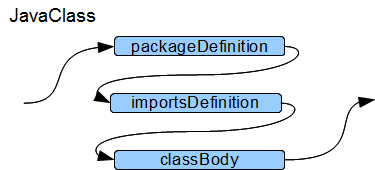
\includegraphics{capitulo09/JavaClass.png}
 \caption{Classe Java}
\end{figure}
% ---------------------------
\subsection{packageDefinition}

\begin{lstlisting}
packageDefinition

   package pathToClass ;
\end{lstlisting}

\begin{figure}[h!]
 \centering
 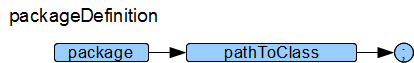
\includegraphics{capitulo09/packageDefinition.png}
 \caption{Definição de pacote}
\end{figure}
% ---------------------------
\subsection{pathToClass}

\begin{lstlisting}
pathToClass

   pathIdentifier
   pathIdentifier . 
\end{lstlisting}

\begin{figure}[h!]
 \centering
 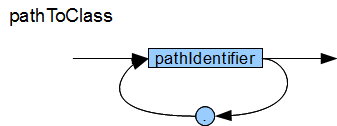
\includegraphics{capitulo09/pathToClass.png}
 \caption{Caminho da classe}
\end{figure}
% ---------------------------
\subsection{pathIdentifier}

\begin{lstlisting}
pathIdentifier

   [a-z]
	
\end{lstlisting}

\begin{figure}[h!]
 \centering
 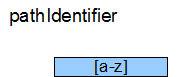
\includegraphics{capitulo09/pathIdentifier.png}
 \caption{Identificador de caminho}
\end{figure}
% ---------------------------
\subsection{importsDefinition}

\begin{lstlisting}
importsDefinition

   import canonicalName ;

\end{lstlisting}

\begin{figure}[h!]
 \centering
 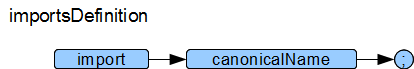
\includegraphics{capitulo09/importsDefinition.png}
 \caption{Definição de import}
\end{figure}
% ---------------------------
\subsection{canonicalName}

\begin{lstlisting}
canonicalName

   pathToClass . ClassName

\end{lstlisting}

\begin{figure}[h!]
 \centering
 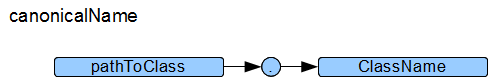
\includegraphics{capitulo09/canonicalName.png}
 \caption{Nome canônico da classe}
\end{figure}
% ---------------------------
\subsection{ClassName}

\begin{lstlisting}
ClassName

   ([A-Z][a-z0-9]+){2,}

\end{lstlisting}

\begin{figure}[h!]
 \centering
 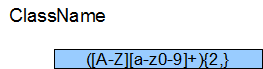
\includegraphics{capitulo09/ClassName.png}
 \caption{Nome da classe}
\end{figure}
% ---------------------------
\subsection{classBody}

\begin{lstlisting}
classBody

   public class ClassName { members }

\end{lstlisting}

\begin{figure}[h!]
 \centering
 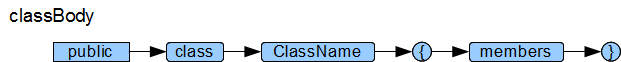
\includegraphics{capitulo09/classBody.png}
 \caption{Declaração de corpo da classe}
\end{figure}
% ---------------------------
\subsection{members}

\begin{lstlisting}
members

   []
   attribute
   method

\end{lstlisting}

\begin{figure}[h!]
 \centering
 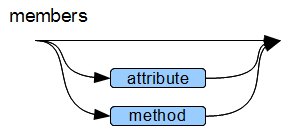
\includegraphics{capitulo09/members.png}
 \caption{Membros da classe}
\end{figure}
% ---------------------------
\subsection{attribute}

\begin{lstlisting}
attribute

   accessor modifier variable ;

\end{lstlisting}

\begin{figure}[h!]
 \centering
 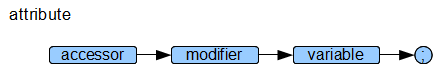
\includegraphics{capitulo09/attribute.png}
 \caption{Atributos}
\end{figure}
% ---------------------------
\subsection{accessor}

\begin{lstlisting}
accessor

   public
   private
   protected
   "default"

\end{lstlisting}

\begin{figure}[h!]
 \centering
 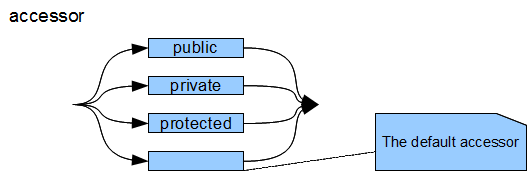
\includegraphics{capitulo09/accessor.png}
 \caption{Acessores}
\end{figure}
% ---------------------------
\subsection{modifier}

\begin{lstlisting}
modifier

   modifier
   modifier modifier
   static
   final

\end{lstlisting}

\begin{figure}[h!]
 \centering
 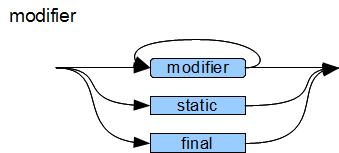
\includegraphics{capitulo09/modifier.png}
 \caption{Modificadores}
\end{figure}
% ---------------------------
\subsection{variable}

\begin{lstlisting}
variable

   type typeName

\end{lstlisting}

\begin{figure}[h!]
 \centering
 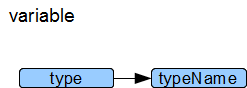
\includegraphics{capitulo09/variable.png}
 \caption{Variável}
\end{figure}
% ---------------------------
\subsection{type}

\begin{lstlisting}
type

   ClassName
   Collection
   primitive

\end{lstlisting}

\begin{figure}[h!]
 \centering
 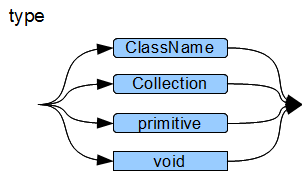
\includegraphics{capitulo09/type.png}
 \caption{Declaração do tipo}
\end{figure}
% ---------------------------
\subsection{primitive}

\begin{lstlisting}
primitive

   byte
   short
   int
   long
   float
   double
   boolean
   char

\end{lstlisting}

\begin{figure}[h!]
 \centering
 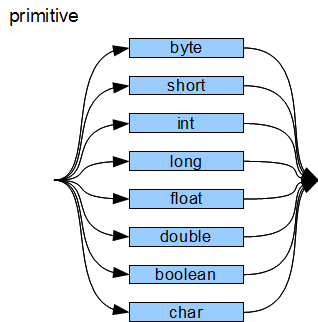
\includegraphics[scale=0.8]{capitulo09/primitive.png}
 \caption{Tipos primitivos}
\end{figure}
% ---------------------------
\subsection{typeName}

\begin{lstlisting}
typeName

   ([a-z0-9][A-Z]+){2,}

\end{lstlisting}

\begin{figure}[h!]
 \centering
 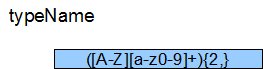
\includegraphics{capitulo09/typeName.png}
 \caption{Nome do tipo}
\end{figure}
% ---------------------------
\subsection{Collection}

\begin{lstlisting}
Collection

   CollectionName < ClassName >

\end{lstlisting}

\begin{figure}[h!]
 \centering
 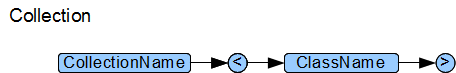
\includegraphics{capitulo09/Collection.png}
 \caption{Definição de coleção}
\end{figure}
% ---------------------------
\subsection{CollectionName}

\begin{lstlisting}
CollectionName

   List
   Set
   Map

\end{lstlisting}

\begin{figure}[h!]
 \centering
 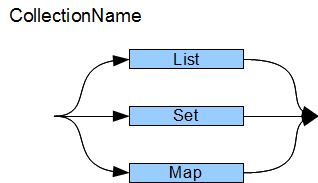
\includegraphics[scale=0.7]{capitulo09/CollectionName.png}
 \caption{Nome da coleção}
\end{figure}
% ---------------------------
\subsection{method}

\begin{lstlisting}
method

   accessor modifier methodIdentifier ( ) { body }
   accessor modifier methodIdentifier ( paramList ) { body }

\end{lstlisting}

\begin{figure}[h!]
 \centering
 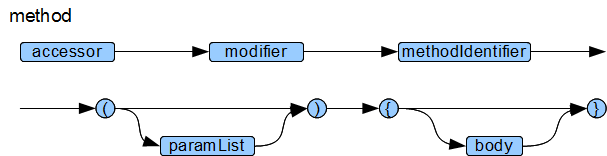
\includegraphics[scale=0.7]{capitulo09/method.png}
 \caption{Definição do método}
\end{figure}
% ---------------------------
\subsection{methodIdentifier}

\begin{lstlisting}
methodIdentifier

   type methodName

\end{lstlisting}

\begin{figure}[h!]
 \centering
 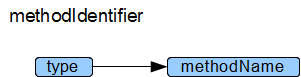
\includegraphics{capitulo09/methodIdentifier.png}
 \caption{Identificação do método}
\end{figure}
% ---------------------------
\subsection{methodName}

\begin{lstlisting}
methodName

   ([a-z0-9][A-Z]+){2,}

\end{lstlisting}

\begin{figure}[h!]
 \centering
 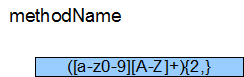
\includegraphics{capitulo09/methodName.png}
 \caption{Nome do método}
\end{figure}
% ---------------------------
\subsection{paramList}

\begin{lstlisting}
paramList

   variable
   variable ,

\end{lstlisting}

\begin{figure}[h!]
 \centering
 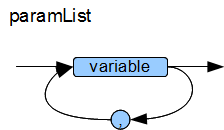
\includegraphics{capitulo09/paramList.png}
 \caption{Lista de parâmetros}
\end{figure}
% ---------------------------
\subsection{body}

\begin{lstlisting}
body

   ""
   statement

\end{lstlisting}

\begin{figure}[h!]
 \centering
 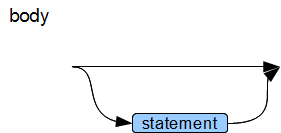
\includegraphics{capitulo09/body.png}
 \caption{Corpo do método}
\end{figure}
% ---------------------------
\subsection{statement}

\begin{lstlisting}
statement

   objectCreation ;
   operationCall ;
   returnStatement ;

\end{lstlisting}

\begin{figure}[h!]
 \centering
 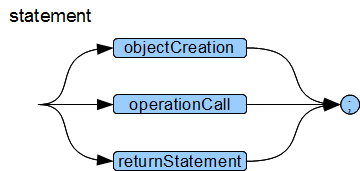
\includegraphics{capitulo09/statement.png}
 \caption{Comandos do método}
\end{figure}
% ---------------------------
\subsection{objectCreation}

\begin{lstlisting}
objectCreation

   ClassName typeName = new ClassName ( )
   ClassName typeName = new ClassName ( paramList )

\end{lstlisting}

\begin{figure}[h!]
 \centering
 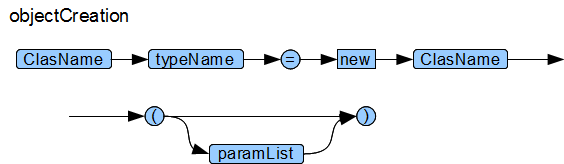
\includegraphics{capitulo09/objectCreation.png}
 \caption{Criação de um objeto}
\end{figure}
% ---------------------------
\newpage
\subsection{operationCall}

\begin{lstlisting}
operationCall

	typeName . methodName ( )
	typeName . methodName ( variableValue )
	typeName . methodName ( variableValue , )

\end{lstlisting}

\begin{figure}[h!]
 \centering
 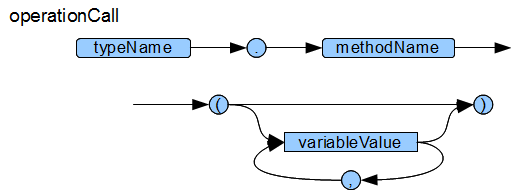
\includegraphics{capitulo09/operationCall.png}
 \caption{Chamada de um métodos}
\end{figure}
% ---------------------------
\subsection{returnStatement}

\begin{lstlisting}
returnStatement

    return type

\end{lstlisting}

\begin{figure}[h!]
 \centering
 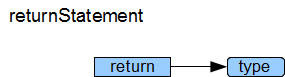
\includegraphics{capitulo09/returnStatement.png}
 \caption{Comando de retorno}
\end{figure}